\documentclass[10pt,a4paper,spanish]{article}

\usepackage[T1]{fontenc} 
\usepackage[utf8]{inputenc}
\usepackage[spanish]{babel}

\usepackage{graphicx}
\usepackage{epstopdf}

\usepackage[export]{adjustbox}
\usepackage{caption}
\usepackage{colortbl} 
\usepackage{dashrule} 
\usepackage{fancyhdr}
\usepackage{float}
\usepackage{framed}
\usepackage[bmargin=2cm,footnotesep=1cm,tmargin=2cm]{geometry} 
\usepackage[pdftex,colorlinks,backref,bookmarks=true,bookmarksnumbered=true,linkcolor=black,urlcolor=black,citecolor=black]{hyperref}
\usepackage[section]{placeins}
\usepackage[labelsep=quad,indention=10pt]{subfig}
\usepackage[spanish,shadow,textsize=small]{todonotes}
\usepackage{wrapfig}
\usepackage{fancyvrb}
\usepackage{xcolor}

% TITULOS
\newcommand{\asig}{Algoritmos y Estructuras de Datos}
\newcommand{\anno}{3º}
\newcommand{\grado}{Grado en Ingeniería Biomédica}
\newcommand{\upm}{Universidad Politécnica de Madrid}
\newcommand{\curso}{}
\newcommand{\ssg}{Rodrigo García Carmona}
\newcommand{\email}{\href{mailto:rodrigo.garciacarmona@ceu.es}{rodrigo.garcia@upm.es}}
\newcommand{\cabecera}[1]{
  \title{Guion de Prácticas}
  \author{\asig\\ \anno\grado\\ \ceu \\ \ssg} 
  \date{#1}
  \maketitle \thispagestyle{fancy}
}

% NUEVAS TODONOTES
\newcommand{\nota}[2][] {\todo[inline, #1]{#2}}
\newcommand{\corregir}[2][] {\todo[color=red, #1]{#2}}
\newcommand{\finaltodo}[2][] {\todo[color=green!40,fancyline #1]{#2}}
\newcommand{\finalnota}[2][] {\todo[color=green!40, inline #1]{#2}}

% PDF
\hypersetup{
  colorlinks=true,
  linkcolor=blue,
  filecolor=magenta,      
  urlcolor=cyan,
  pdfauthor={\ssg},
  pdftitle={Guion de Prácticas},
  pdfsubject={\asig, \grado, \upm, Madrid, España},
  pdfkeywords={algoritmos, estructuras de datos, ingeniería biomédica, guion, prácticas}, 
  pdftoolbar=true,
  pdfmenubar=true,
  pdffitwindow=true,
  pdfnewwindow=true
}

% ENCABEZADO
\pagestyle{fancy}%
  \renewcommand{\headrulewidth}{0.1pt}
  \renewcommand{\footrulewidth}{0.1pt}
  \fancyhf{}
  \fancyhead[L]{
\includegraphics[width=8mm]{templates/ETSIT-UPM.eps}}
  \fancyhead[C]{\small{\asig}\\\small{\grado}}
  \fancyhead[R]{\curso}
  \fancyfoot[L]{}
  \fancyfoot[C]{\thepage}
  \fancyfoot[R]{}

% CAJA SOMBREADA
% comando \sombreado{Título}{Texto}
\definecolor{shadecolor}{rgb}{0.9,0.9,0.9}
\newcommand{\sombreado}[2]{
  \begin{shaded}
    \begin{center} \emph{\textsc{#1}} \end{center}
    \noindent #2\\
  \end{shaded}
}

% CAJA INSTRUCCIONES 
\definecolor{shadecolor}{rgb}{0.9,0.9,0.9}
\newcommand{\instrucciones}[7]{
  \begin{shaded}
    \begin{center} \emph{\textsc{#1}}
    \end{center}
    %\noindent \emph{\textsc{Fecha límite de entrega: }} \emph{#4}\\
    %\emph{\textsc{Peso: }}\emph{#5}\newline\newline
    #6

    #7
  \end{shaded}
}

% Código fuente
\newcommand{\code}[1]{\texttt{#1}}

% Big O
\newcommand{\bigO}{\mathcal{O}}


% Minted
\usepackage{minted}
% Optional: Set a default style. 'manni' is a light, clean style.
% Other popular styles include 'tango', 'monokai', 'solarized-light'.
\usemintedstyle{sas}

% PRACTICA
\newcommand{\practica}{Práctica 3: Búsqueda}
\newcommand{\notaob}{
\begin{center}
Rodrigo García Carmona\footnotemark\\
\href{mailto:rodrigo.garcia@upm.es}{rodrigo.garcia@upm.es}\\

\includegraphics[width=20mm]{templates/by-nc-sa.eps}
\end{center}

Esta práctica es individual y sirve tanto para desarrollar como para poner a prueba los conocimientos adquiridos. Realizar esta práctica es recomendable para aumentar las probabilidades de éxito en los exámenes teóricos.
}

% MACROS

% CONTENIDO
\begin{document}

\instrucciones{\practica}{\tiempo}{\obligatoria}{\fecha}{\peso}{\notaob}

\section{Preparación de la práctica}
\footnotetext{Desarrollada a partir del trabajo previo de Miguel Ángel de Miguel.}

El objetivo de esta práctica es entender la diferencia entre la búsqueda lineal (por fuerza bruta) y otros algoritmos de búsqueda más eficientes que, sin embargo, requieren de una ordenación previa de los datos. También busca poner en práctica el análisis de algoritmos para entender la complejidad computacional. Se estudiarán los siguientes conceptos:

\begin{itemize}
    \item Implementación de una búsqueda lineal.
    \item Análisis de la complejidad computacional (usando la notación $\bigO$).
    \item Comprensión de un proceso de ordenación.
    \item Implementación de una búsqueda binaria.
    \item Medida de rendimiento.
\end{itemize}

\sombreado{Trabajo previo al laboratorio}{El tiempo de las clases de laboratorio es muy valioso, ya que en ellas tendrá a su disposición a los profesores para resolver cualquier duda que le pueda surgir. Por tanto, para facilitar al máximo el aprovechamiento de este tiempo, las prácticas se han dividido en varias secciones. La primera de ellas (``preparación de la práctica'') puede ¡y debe! realizarse \textbf{antes de la sesión de laboratorio} propiamente dicha. Leer esta sección antes de entrar a clase hará que su tiempo en el laboratorio sea más productivo y provocará que las dudas más importantes le surjan \textbf{durante la clase}, y \textbf{no después}, cuando se encuentre estudiando solo en su casa y la única opción que le quede sea escribir un email al profesor.

De hecho, es especialmente importante evitar que se den situaciones como esta la noche antes de un examen.}

\subsection{Secuenciación del genoma}

Uno de los grandes retos de la medicina moderna es dar sentido a la enorme cantidad de información codificada en el genoma de los seres vivos, ya sean estos personas, animales, plantas, bacterias o incluso virus. Este problema, que a primera vista podría parecer puramente biológico, tiene un componente enormemente importante de procesado de datos.

De hecho, es un ejemplo paradigmático de la utilidad de las técnicas de ``Big Data''; es decir, del manejo de enormes volúmenes de datos. Hay que tener presente que el genoma de cada ser humano contiene, en sus 23 cromosomas, más de 3.000 millones de pares de bases de ADN.

El proceso de secuenciación de ADN (o ARN) consiste en la identificación, a partir de una muestra biológica (que en el caso del ser humano puede ser sangre, saliva o tejidos), de una secuencia de nucleótidos que, si estamos hablando del ADN, pueden tener cada uno una de las siguientes cuatro bases:

\begin{itemize}
    \item \textbf{A:} Adenina
    \item \textbf{G:} Guanina
    \item \textbf{C:} Citosina
    \item \textbf{T:} Timina
\end{itemize}

Desgraciadamente, las tecnologías de secuenciación actuales no pueden leer una secuencia de nucleótidos tan larga como la del ser humano de principio a fin. El ADN de un genoma con miles de millones de pares de bases es una molécula demasiado larga para que una sola máquina lo lea de una sola vez. Por tanto, el ADN se rompe primero en muchos fragmentos más pequeños, llamados ``lecturas'', que pueden ser más cortos (cientos de pares de bases por lectura) o más largos (decenas de miles de pares de bases por lectura). Por ejemplo, el secuenciador Illumina HiSeq, que aparece en la Figura \ref{fig:sequencer}, puede leer hasta 2x250 pares de bases (250 desde el inicio del fragmento y 250 desde el final).

\begin{figure}[!htbp]
  \centering
  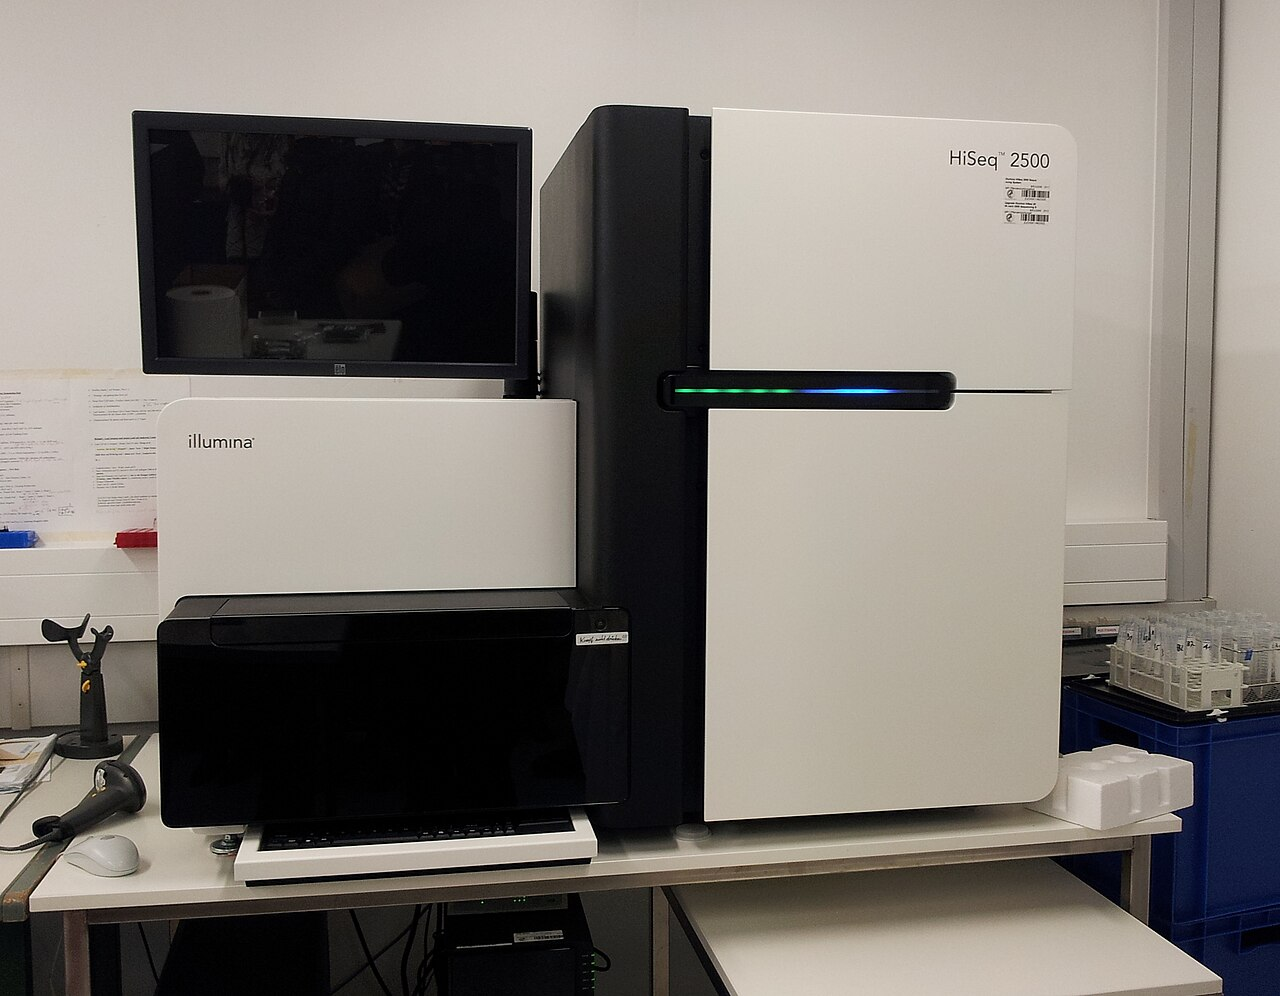
\includegraphics[width=\textwidth]{files/Illumina_HiSeq_2500.jpg}
  \caption{Secuenciador Illumina HiSeq 2500}
  \label{fig:sequencer}
\end{figure}

\subsection{Búsqueda de secuencias}
\label{sec:modelos}

Así pues, uno de los problemas más comunes de la bioinformática consiste en tomar estos millones de lecturas y encontrar el lugar en el que encajan dentro del genoma en su conjunto. Este proceso no es sino una búsqueda, y la eficiencia con la que se realice es crítica: una diferencia de tan solo unas decenas milisegundos para cada lectura se traduce en días o semanas de tiempo de cómputo.

La búsqueda de secuencias resulta fundamental en aplicaciones como el ensamblaje de genomas (a partir de fragmentos), la detección de secuencias genéticas específicas, las comparaciones genómicas, el análisis de proteínas y los estudios genéticos individualizados. Este tipo de tareas se llevan a cabo en campos muy dispares (no solo la medicina), como puede ser la criminología o la antropología.

Esto es posible debido a la existencia de un modelo de referencia del genoma humano, una herramienta indispensable para el campo de la genómica y uno de los mayores logros científicos de la humanidad. El modelo de referencia más usado, que contiene la secuencia estándar de los 23 cromosomas del ser humano, recibe el nombre de GRCh38 (Genome Reference Consortium human build 38) y puede descargarse \href{https://hgdownload.cse.ucsc.edu/downloads.html#human}{de la web de la Universidad de California en Santa Cruz}.

Sí, vivimos en un mundo en el que uno se puede descargar el genoma humano a través de Internet.

\sombreado{Otros modelos de referencia}{El GRCh38 es el modelo tradicionalmente más usado, y continuamente se están publicando parches sobre el mismo (el último es el p14) para corregir errores y rellenar huecos. Sin embargo, no es el único modelo que existe y, de hecho, el honor de ser el primer genoma completo del ser humano le corresponde al modelo T2T-CHM13 (Telomere-to-Telomere Consortium CHM13), que cerró huecos importantes en los centrómeros y otras regiones repetitivas que el GRCh38 aún tenía. El modelo T2T-CHM134 está disponible (además de en la web de la Universidad de California en Santa Cruz), curiosamente, \href{https://github.com/marbl/CHM13}{también en GitHub}. Dicho esto, aunque el T2T-CHM134 es más reciente y completo que el GRCh38, este último tiene más información funcional y biológica ya validada por la comunidad científica, por lo que se usa mucho.

En la actualidad se está trabajando en la creación del HPRC (Human Pangenome Reference Consortium), una colección de genomas (un pangenoma) que combina las secuencias de miles de individuos lo más diversos posibles, para así poder capturar la gran variedad de características genéticas que existe en la especie humana. Esta iniciativa nació porque los modelos de referencia actualmente existentes solo modelan el genoma de unos pocos individuos que, además, son mayormente de ascendencia europea.}

\subsection{Aplicaciones de la búsqueda de secuencias}

La búsqueda de secuencias específicas dentro del genoma tiene muchas aplicaciones en el campo de la ingeniería biomédica. Sin ser exhaustivos:

\begin{itemize}
    \item \textbf{Diagnóstico de enfermedades genéticas:} muchas enfermedades, como la fibrosis quística o la anemia de células falciformes, son causadas por mutaciones muy específicas en un gen conocido. Por ejemplo, la fibrosis quística a menudo se debe a una mutación en el gen CFTR.
    Por tanto, un médico que sospeche de que un paciente posee esta enfermedad podría solicitar la secuenciación de su gen CFTR, obteniendo la respuesta a si la mutación está presente.
    \item \textbf{Oncología:} Ciertas mutaciones en genes como el BRCA1 (asociado al cáncer de mama) o el EGFR (asociado al cáncer de pulmón) no solo indican un mayor riesgo de padecer enfermdades, sino que también sirven para predecir qué fármacos serán más efectivos. Tras secuenciar el ADN de un tumor, se buscan mutaciones para las que existe una terapia dirigida, mucho más eficaz y con menos efectos secundarios que la quimioterapia tradicional.
    \item \textbf{Predicción de la respuesta a fármacos:} A veces un medicamento es eficaz en una persona y no en otra. Esto puede deberse a las diferencias genéticas, pues algunas variantes (como la familia de genes CYP450, que codifica enzimas hepáticas) determinan cómo se metabolizan varios fármacos comunes. Si esto se conoce con antelación, se podría ajustar la dosis o elegir un fármaco alternativo desde el principio, evitando un largo y tortuoso proceso de prueba y error.
    \item \textbf{Ensamblado de genomas \textit{de novo}:} El proceso de creación de un genoma de referencia para una especie se denomina ensamblado \textit{de novo}. En este proceso lo que se buscan son solapamientos, de tal manera que se puedan encajar unos fragmentos con otros hasta que, finalmente, se obtienen los cromosomas completos.
\end{itemize}

En todos estos casos el proceso al final es el mismo: se parte de una secuencia de bases y se busca encontrar en qué puntos del genoma aparece dicha secuencia. Si, por ejemplo, el propósito de un análisis es reconstruir la secuencia genómica de un individuo, lo que se hace es comparar las secuencias extraídas con las del modelo de referencia del genoma humano. Para ello es necesario encontrar el punto en el que encaja cada secuencia. Una vez hecho esto, se pueden analizar las variaciones propias del sujeto analizado y encontrar la mutación o característica específica que estemos buscando.

\sombreado{El maldito COVID}{Si ha cotilleado en la página de la Universidad de California en Santa Cruz habrá visto que, además del genoma humano, también puede descargar otros genomas, entre ellos el del infame SARS-CoV-2, el causante del maldito COVID.

Poco después del inicio de la epidemia, científicos chinos secuenciaron el genoma del SARS-CoV-2 e hicieron públicos los datos, lo que permitió a investigadores de todo el mundo estudiar la composición genética del virus. Esta secuenciación temprana reveló la alta similitud entre el SARS-CoV-2 y los coronavirus de murciélago.

Los datos genómicos también ayudaron a rastrear la propagación del virus e identificar las rutas de transmisión. Por ejemplo, la secuenciación de los primeros casos de SARS-CoV-2 en Ecuador mostró que el virus estaba estrechamente relacionado con cepas de los Países Bajos. Además, la secuenciación rápida permitió la detección de la variante Ómicron a las pocas horas de recibir una muestra de un viajero que regresaba de Sudáfrica. Estos esfuerzos han permitido a los científicos monitorizar mutaciones, seguir las cadenas de transmisión y permitir a la sociedad prepararse y luchar contra este virus.}

\subsection{Los archivos FASTA}

Si uno se descarga un modelo genético, por ejemplo, \href{https://hgdownload.cse.ucsc.edu/goldenPath/hg38/chromosomes/chr13.fa.gz}{el del cromosoma 13 del modelo de referencia GRCh38}, lo más habitual es que se encuentre las secuencias correspondientes en un formato de archivo llamado \href{https://en.wikipedia.org/wiki/FASTA_format}{FASTA}, que no es más que un archivo de texto en el que cada base está identificada por su primera letra (en mayúsculas o minúsculas, indistintamente), almacenada usando un \textit{byte}. De esta forma, el texto \code{GATTACA} (de 7 \textit{bytes}) corresponderá a la secuencia de bases ``Guanina-Adenina-Timina-Timina-Adenina-Citosina-Adenina''. Estos archivos, además, tienen saltos de líneas a intervalos constantes para facilitar la lectura, que deben de ser ignorados a la hora de procesarlos. Por último, es importante tener en cuenta que la primera línea de estos archivos, que empieza por el carácter ``\code{>}'', también debe ser ignorada, pues contiene un comentario.

A continuación tiene un ejemplo del comienzo de un archivo FASTA:

\begin{verbatim}
>chr19 Homo sapiens isolate
GATCACAGAGGCTGGGCTGCTCCCCACCCTCTGCACACCTCCTGCTTCTA
ACAGCAGAGCTGCCAGGCCAGGCCCTCAGGCAAGGGCTCTGAAGTCAGGG
TCACCTACTTGCCAGGGCCGATCTTGGTGCCATCCAGGGGGCCTCTACAA
GGATAATCTGACCTGCAGGGTCGAGGAGTTGACGGTGCTGAGTTCCCTGC
ACTCTCAGTAGGGACAGGCCCTATGCTGCCACCTGTACATGCTATCTGAA
GGACAGCCTCCAGGGCACACAGAGGATGGTATTTACACATGCACACATGG
CTACTGATGGGGCAAGCACTTCACAACCCCTCATGATCACGTGCAGCAGA
...
\end{verbatim}

\sombreado{Archivos .gz}{Habrá observado que el archivo que ha descargado pesa casi 1 GB. Bueno, pues, a pesar de todo, es un archivo comprimido. Eso es, precisamente, lo que indica la extensión ``gz'' al final del mismo. Si quiere, puede descomprimirlo usando 7Zip u otra herramienta similar. Al hacerlo, comprobará que el archivo de texto pesa aún más; en este caso, pasa de los 3 GB.}

En muchos archivos FASTA, además de los habituales `A', `C', `G' y `T' (y `U' en el caso del ARN) también veremos el carácter `N' para indicar los nucleóticos indefinidos. Esta letra significa ``cualquiera de las cuatro bases'', y suele aparecer en secuencias de bases desconocidas o de alta variabilidad. Estas regiones, por lo general, no tienen un efecto conocido sobre el desarrollo humano.

\subsection{Objetivo y descarga de la práctica}

El objetivo de la práctica es buscar varias secuencias cortas de bases en el modelo de referencia humano. Implementará varias versiones de dos algoritmos de búsqueda (lineal y binaria) y comparará el rendimiento de todos ellos. Al final de la práctica entenderá la utilidad de los algoritmos de búsqueda y ordenación a través de una aplicación real. O eso espera su profesor; así que, por favor, no le defraude.

La práctica está disponible en GitHub, en la siguiente dirección de Internet (URI):

\href{https://github.com/rgarciacarmona/ALED-lab3}{https://github.com/rgarciacarmona/ALED-lab3}

Para trabajar en ella, siga estos pasos:

\begin{enumerate}
    \item Haga un \textit{fork} de este repositorio a su cuenta de GitHub.
    \item Antes de empezar a hacer \textit{commits}, compruebe en \textit{Settings $\to$ General} de su \textit{fork} que la visibilidad es \textbf{pública}. Solo se evaluarán los \textit{commits} hechos sobre un \textit{fork} público.
    \item Clone su \textit{fork} e impórtelo en Eclipse. Para ello, seleccione \textit{File $\to$ Import...} y, de entre las opciones disponibles, \textit{Git $\to$ Projects from Git $\to$ Clone URI}. A continuación, introduzca la URI de su \textit{fork} (\texttt{https://github.com/}\textit{usuario}\texttt{/ALED-lab3}, donde \textit{usuario} es su nombre de usuario de GitHub), no la del repositorio original. Después, haga click en \textit{Next} tantas veces como sea necesario y, por último, en \textit{Finish}.
    \item Trabaje, haga \textit{commit} de sus cambios y haga \textit{push} a su \textit{fork}.
\end{enumerate}

Tómese su tiempo para examinar todas las clases del proyecto que acaba de importar. Intente figurarse, a base de observar el código, para qué sirve cada una de ellas.

\subsection{Estructura del proyecto Java}

Una vez descargado el código de la práctica, verá que este está compuesto únicamente de cinco clases, divididas en dos paquetes:

\begin{itemize}
    \item \code{es.upm.aled.lab3}: Que contiene las clases necesarias para implementar una búsqueda lineal.
    \item \code{es.upm.aled.lab3.binary}: Que contiene las clases necesarias para implementar una búsqueda binaria.
\end{itemize}

Como en el resto de prácticas, habrá parte del código de estas clases que tendrá que completar usted. Por el momento, ignore el paquete \code{es.upm.aled.lab3.binary}, ya que todavía no va a trabajar con él. 

Fíjese en el paquete \code{es.upm.aled.lab3}, que contiene únicamente dos clases:

\begin{itemize}
    \item \code{FASTAException}, que es una clase hija de \code{Exception} cuyo propósito es identificar que una excepción tiene su origen en el procesado de los datos obtenidos a partir de un archivo FASTA.
    \item \code{FASTAReader}, que es la clase sobre la que trabajará en las secciones \ref{sec:laboratorio} y \ref{sec:laboratorio2} de la práctica. Este clase permite buscar secuencias de ADN en un genoma.
\end{itemize}

Dedique algo de tiempo a entender cómo funciona la clase \code{FASTAReader} y \textbf{responda a las siguientes preguntas:}

\begin{itemize}
    \item ¿Qué hacer el método \code{search()} de la clase {FASTAReader}? ¿Qué devuelve?
    \item ¿Qué argumentos tendrá el método \code{main()}? ¿Qué función tiene cada uno?
    \item Abra la carpeta \code{cromosomes} y observe los archivos que tiene dentro. ¿En qué formato están? ¿Qué información contienen?
\end{itemize}

\subsection{Construcción de la estructura de datos}

Si ha estudiado el código de \code{FASTAReader} habrá observado que esta clase tiene dos atributos:

\begin{minted}[
  frame=lines, % Adds a frame around the code
  framesep=2mm,
  % linenos % Enables line numbers
]{java}
protected byte[] content;
protected int validBytes;
\end{minted}

El primero de ellos, \code{content}, es un \code{array} de \code{bytes} que contiene la secuencia completa de nucleótidos de un archivo FASTA. Este será nuestro genoma.

El segundo, \code{validBytes}, indica cuántos de los \code{bytes} de \code{content} son válidos. Es decir, que solo serán válidos los elementos desde  \code{content[0]} hasta \code{content[validBytes - 1]}. Este \code{validBytes} es necesario porque los ficheros FASTA incluyen algunos caracteres que no nos interesan (por ejemplo, saltos de línea), pero antes de leer el fichero no podemos saber cuántos de esos caracteres nos encontraremos y, por tanto, no podemos conocer con exactitud cuál debería ser el tamaño concreto del \code{array}. Solo obtendremos esta información tras haber finalizado la lectura del archivo, momento en el que ya habremos rellenado \code{content} con los datos que nos interesan. Llegados a ese punto, la única forma de tener un \code{array} de tamaño exacto sería hacer una copia a otro \code{array} más pequeño, del tamaño deseado. Este es un proceso con un coste de $\bigO(n)$, que se añade a la complejidad de todo el resto del algoritmo, por es preferible evitarlo si no es necesario.

Puede ver todo el proceso de inicialización de estos dos atributos en el método \code{readFile()}.

\sombreado{¿Por qué byte y no char?}{Quizá se esté preguntando por qué \code{content} es un \code{array} de \code{bytes} y no de \code{chars}. Esto se debe a que en los archivos FASTA cada base se almacena como un carácter en formato ASCII, que ocupa un \textit{byte}. Por su parte, en Java, cada \code{char} ocupa 2 \textit{bytes}, porque usa el estándar UTF-16.}

\subsection{Búsqueda lineal de secuencias}

Antes de implementar una búsqueda lineal de secuencias en un genoma es necesario entender bien qué se está haciendo. Los puntos clave son, resumiendo, los dos siguientes:

\begin{enumerate}
    \item La secuencia \textbf{entera} debe coincidir.
    \item Deben devolverse \textbf{todos aquellos puntos del genoma} en los que aparezca la secuencia. No solo el primero (o uno de ellos al azar).
\end{enumerate}

A continuación se detalla un ejemplo que ilustra este proceso: se desea buscar el patrón \code{GATTACA} dentro del siguiente genoma:

\begin{center}
\begin{verbatim}
T G A T T A C A G A T T A C A
\end{verbatim}
\end{center}

Como se trata de una búsqueda lineal, iremos comparando el patrón con el genoma, posición a posición:

\newcommand{\red}[1]{\textcolor{red}{#1}}
\newcommand{\blue}[1]{\textcolor{blue}{#1}}

\begin{center}
\begin{tabular}{|*{15}{c|}}
\hline
0 & 1 & 2 & 3 & 4 & 5 & 6 & 7 & 8 & 9 & 10 & 11 & 12 & 13 & 14 \\
\hline
T & G & A & T & T & A & C & A & G & A & T & T & A & C & A \\
\hline
\red{G} & \red{A} & \red{T} & \red{T} & \red{A} & \red{C} & \red{A} & & & & & & & & \\
\hline
\end{tabular}
\end{center}

En la posición 0 \textbf{no hay} coincidencia. Probamos con la siguiente:

\begin{center}
\begin{tabular}{|*{15}{c|}}
\hline
0 & \blue{1} & 2 & 3 & 4 & 5 & 6 & 7 & 8 & 9 & 10 & 11 & 12 & 13 & 14 \\
\hline
T & \blue{G} & \blue{A} & \blue{T} & \blue{T} & \blue{A} & \blue{C} & \blue{A} & G & A & T & T & A & C & A \\
\hline
& \red{G} & \red{A} & \red{T} & \red{T} & \red{A} & \red{C} & \red{A} & & & & & & & \\
\hline
\end{tabular}
\end{center}

En la posición 1 \textbf{sí hay} coincidencia. Probamos con la siguiente:

\begin{center}
\begin{tabular}{|*{15}{c|}}
\hline
0 & 1 & 2 & 3 & 4 & 5 & 6 & 7 & 8 & 9 & 10 & 11 & 12 & 13 & 14 \\
\hline
T & G & A & T & T & A & C & A & G & A & T & T & A & C & A \\
\hline
& & \red{G} & \red{A} & \red{T} & \red{T} & \red{A} & \red{C} & \red{A} & & & & & & \\
\hline
\end{tabular}
\end{center}

En la posición 2 \textbf{no hay} coincidencia. Vemos que \textbf{tampoco habrá} en las posiciones 3, 4, 5, 6 y 7. Probamos con la posición 8:

\begin{center}
\begin{tabular}{|*{15}{c|}}
\hline
0 & 1 & 2 & 3 & 4 & 5 & 6 & 7 & \blue{8} & 9 & 10 & 11 & 12 & 13 & 14 \\
\hline
T & G & A & T & T & A & C & A & \blue{G} & \blue{A} & \blue{T} & \blue{T} & \blue{A} & \blue{C} & \blue{A} \\
\hline
& & & & & & & & \red{G} & \red{A} & \red{T} & \red{T} & \red{A} & \red{C} & \red{A} \\
\hline
\end{tabular}
\end{center}

Aquí si vuelve a coincidir. Por tanto, el resultado de la búsqueda serán las posiciones 1 y 8.

Enhorabuena, ya ha terminado con el trabajo previo a la sesión de laboratorio. Las secciones de la \ref{sec:laboratorio} en adelante puede realizarlas en clase.

\section{Implementación de una búsqueda lineal de secuencias}
\label{sec:laboratorio}

Ahora que ya sabe cómo funciona la búsqueda lineal (también llamada ``por fuerza bruta'') de secuencias en un genoma, impleméntela. Complete el método \code{search()} de la clase \code{FASTAReader}. Para implementar este método tenga en cuenta que debe usar el método \code{compare()}, que ya se le proporciona hecho y cuyo contenido se reproduce a continuación:


\begin{minted}[
  frame=lines, % Adds a frame around the code
  framesep=2mm,
  % linenos % Enables line numbers
]{java}
/*
 * Helper method that checks if a pattern appears at a specific position in the
 * data array. It checks every byte of the pattern one by one. If the pattern
 * length would need to access a position after the valid bytes of the array, it
 * throws a new FASTAException to indicate this fact.
 * 
 * Returns true if the pattern is present at the given position; false
 * otherwise.
 */
private boolean compare(byte[] pattern, int position) throws FASTAException {
    if (position + pattern.length > validBytes) {
        throw new FASTAException("Pattern goes beyond the end of the file.");
    }
    boolean match = true;
    for (int i = 0; i < pattern.length; i++) {
        if (pattern[i] != content[position + i]) {
            match = false;
        }
    }
    return match;
}
\end{minted}

Fíjese en particular en que este método lanza una \code{FASTAException} cuando se está intentando buscar el patrón más allá de los \textit{bytes} válidos. Así, pues, cuando use el método \code{compare()} deberá estar preparado para, si se produce esta excepcíon, capturarla y terminar con la búsqueda, pues este hecho indicará que se ha llegado al final de los datos.

\subsection{Prueba de la búsqueda lineal}

Para probar el código que acaba de implementar, deberá crear una nueva configuración de lanzamiento con las siguientes características (consulte la Práctica 1 si no sabe qué es nada de esto):

\begin{itemize}
    \item Ejecute el método \code{main} de la clase {FASTAReader}.
    \item Pásele dos argumentos:
    \begin{itemize}
        \item El primero deberá ser el nombre del fichero a procesar: ``cromosomes/chr19segment.fa''
        \item El segundo deberá ser la cadena a buscar: ''GATTACAGACA''
    \end{itemize}
\end{itemize}

Si ha implementado bien la búsqueda lineal, deberá ver en la consola un texto parecido al siguiente (los números de tiempos pueden variar en función de la potencia de su PC):

\begin{verbatim}
Tiempo de apertura de fichero: 556538400
Tiempo de búsqueda: 4994900
Encontrado GATTACAGACA en 418072
Encontrado GATTACAGACA en 497920
Encontrado GATTACAGACA en 500757
Tiempo total: 571101300
\end{verbatim}

Acaba de hacer una búsqueda sobre un pequeño fragmento del cromosoma 19, de tan solo 600 KB. Ahora modifique el primer parámetro para usar el cromosoma 19 completo, que se encuentra en el archivo ``cromosomes/chr19.fa''. Este archivo pesa 60 MB. Esta ejecución le llevará a su PC bastante más tiempo (puede que varios minutos), y deberá producir el siguiente resultado:

\begin{verbatim}
Tiempo de apertura de fichero: 54001829700
Tiempo de búsqueda: 1121731400
Encontrado GATTACAGACA en 232650
Encontrado GATTACAGACA en 1153371
Encontrado GATTACAGACA en 1204888
...
Encontrado GATTACAGACA en 58798540
Encontrado GATTACAGACA en 58872992
Tiempo total: 55136743300
\end{verbatim}

Si quiere, pruebe a descargar otros datos genéticos de los modelos de referencia que se indicaban en la sección \ref{sec:modelos} y a hacer búsquedas sobre ellos.

\sombreado{OutOfMemoryError}{Si al ejecutar su código con el archivo del cromosoma completo (o con otros archivos que haya descargado usted mismo) obtiene un \code{OutOfMemoryError}, tendrá que aumentar la cantidad de memoria que utiliza la máquina virtual de Java. Puede hacerlo escribiendo los argumentos \code{-Xmx2g -Xms512m} en el cuadro \textbf{VM Arguments} de la configuración de lanzamiento. El primero de estos dos argumentos aumenta el tamaño máximo de memoria para nuevos objetos a 2 GB, mientras que el segundo fija el tamaño inicial de este espacio de memoria a 512MB.}

\textbf{Responda a las siguientes preguntas:}

\begin{itemize}
    \item Según la notación $\bigO$, ¿cuál es orden de complejidad del algoritmo de búsqueda que ha implementado?
    \item Compare los tiempos obtenidos al buscar en un archivo de 600 KB con los obtenidos al buscar en un archivo de 60 MB. ¿Son consistentes con el orden del algoritmo?
\end{itemize}

\subsection{Mejora del método \code{compare()}}

Si se fija en la implementación de \code{compare()} que se le ha proporcionado, quizá caiga en la cuenta de que es mejorable; con una pequeña modificación podrían reducirse los tiempos de ejecución.

Observe que la versión actual de este método \textbf{siempre} recorre todo el contenido del
patrón, incluso aunque ya se haya comprobado que el patrón no va a encajar en la secuencia. Por ejemplo, en la siguiente comparación:

\begin{center}
\begin{tabular}{|*{15}{c|}}
\hline
0 & 1 & 2 & 3 & 4 & 5 & 6 & 7 & 8 & 9 & 10 & 11 & 12 & 13 & 14 \\
\hline
T & G & A & T & T & A & C & A & G & A & T & T & A & C & A \\
\hline
& & \red{G} & \red{A} & \red{T} & \red{T} & \red{A} & \red{C} & \red{A} & & & & & & \\
\hline
\end{tabular}
\end{center}

Una vez se ha comprobado la posición 2 del genoma y se ha visto que las dos bases (`A' y `G') no coinciden, no es necesario comprobar las posiciones de la 3 a a la 8. Sin embargo, la implementación de \code{compare()} actual las comprueba todas.

Implemente el método \code{compareImproved()}, que, a diferencia de \code{compare()}, devuelve \code{false} en cuanto una base no coincide. Puede ``inspirarse'' en el código ya existente de \code{compare()}. En cualquier caso, no olvide que tiene que lanzar una \code{FASTAException} si el patrón se extiende más allá de los \textit{bytes} válidos.

A continuación, modifique su método \code{search()} para que use \code{compareImproved()} en lugar de \code{compare()}.

Por último, ejecute de nuevo las dos búsquedas anteriores y compare los nuevos tiempos con los que obtuvo anteriormente.

\textbf{Responda a las siguientes preguntas:}

\begin{itemize}
    \item Según la notación $\bigO$, ¿ha cambiado el orden de complejidad del algoritmo tras este cambio?
    \item Compare los tiempos obtenidos al buscar en un archivo de 600 KB con los obtenidos al buscar en un archivo de 60 MB. ¿Son consistentes con el orden del algoritmo?
    \item ¿Ha mejorado el caso peor de la búsqueda, o únicamente el caso medio?
\end{itemize}

\section{Soporte para SNV}
\label{sec:laboratorio2}

En ocasiones, la secuencia extraída por un secuenciador puede no ser idéntica a otra secuencia presente en el cromosoma. Estas pequeñas variaciones son producidas por el proceso de formación de células, errores en el proceso de secuenciación, imperfecciones en el modelo de referencia o efectos externos, entre otros.

Se desea expandir el código de la práctica para que soporte un tipo de variaciones conocidas como SNV (\textit{Single Nucleotide Variant}), en las que se permite una diferencia de \textbf{una} base entre la secuencia y el genoma de referencia. Por ejemplo, en el siguiente caso, si se soportara SNV:

\begin{center}
\begin{tabular}{|*{15}{c|}}
\hline
0 & \blue{1} & 2 & 3 & 4 & 5 & 6 & 7 & 8 & 9 & 10 & 11 & 12 & 13 & 14 \\
\hline
T & \blue{G} & \blue{A} & \blue{T} & A & \blue{A} & \blue{C} & \blue{A} & G & A & T & T & A & C & A \\
\hline
& \red{G} & \red{A} & \red{T} & \red{T} & \red{A} & \red{C} & \red{A} & & & & & & & \\
\hline
\end{tabular}
\end{center}

Debería aceptarse el índice 1 como una coincidencia, a pesar de que una de las 7 bases comparadas (la 4) no coincide.

Ahora va a añadir esta funcionalidad a la clase \code{FASTAReader}. En primer lugar, implemente el método \code{compareNumErrors()}, similar al \code{compare()} que ya había implementado antes, pero con el siguientes cambio: en lugar de \code{true} o \code{false}, este método debe devolver un \code{int} con el número de bases en las que difiere el patrón de la posición indicada en el genoma:

\begin{minted}[
  frame=lines, % Adds a frame around the code
  framesep=2mm,
  % linenos % Enables line numbers
]{java}
/*
 * Improved version of the compare method that returns the number of bytes in
 * the pattern that are different from the ones present in the data array at the
 * given position.
 * 
 * Returns the number of characters in the pattern that are different from the
 * ones present in the indicated position.
 */
private int compareNumErrors(byte[] pattern, int position) throws FASTAException {
    // TODO
    return null;
}
\end{minted}

Después, implemente el método \code{searchSNV()}, que debe usar el método \code{compareNumErrors()} que acaba de crear para obtener el número de diferencias entre un patrón y una posición del genoma y, si este número es 0 (coincidencia exacta) o 1, añadir la posición a la lista de enteros a devolver.

Por último, modifique el método \code{main()} de \code{FASTAReader} para que use \code{searchSNV()}. Realice de nuevo las dos búsquedas anteriores.

\textbf{Responda a las siguientes preguntas:}

\begin{itemize}
    \item Según la notación $\bigO$, ¿ha cambiado el orden de complejidad del algoritmo tras este cambio?
    \item ¿Ha cambiado apreciablemente el tiempo de ejecución?
\end{itemize}

\section{Implementación de una búsqueda binaria}

Como ya sabe por las clases teóricas, para poder hacer una búsqueda binaria primero es necesario tener un conjunto de datos ordenados. Ahora que ha recordado este detalle tan importante, reflexione un momento sobre qué puede significar que los datos estén ``ordenados'' en una secuencia de ADN. Lógicamente, no podemos cambiar el orden de las bases del genoma ni del patrón, sino que lo que tenemos que hacer es otra cosa.

Pensemos en qué estamos buscando: una cadena de caracteres (el patrón). Ahora pensemos en dónde la estamos buscando: dentro de otra cadena de caracteres más grande (el genoma). Por tanto, una forma de ``ordenar'' este genoma es crear un glosario (como el que se encuentra al final de un libro de texto) que nos permita saber en qué punto (el índice) del genoma se encuentran todas y cada una de las subcadenas de caracteres que lo conforman. Este glosario hipotético tendría, por tanto, una entrada para cada cadena de caracteres contenida en el genoma, seguida de los índices (puede haber más de uno) en los que se encuentra presente dicha cadena.

Esta idea, aunque teóricamente buena, es impracticable, porque tendríamos que tener un glosario con, si el tamaño del genoma es de $n$ bases, $n\times(n+1)/2$ entradas. Es decir, que para el genoma de un fichero de 60 MB (como el que ha estado usando), necesitaríamos un glosario de aproximadamente 3.600 TB (3,6 PB).

Pero no desespere, aunque esta estrategia sea impracticable, lo que sí podemos es tener un glosario de sufijos, siendo un sufijo el resultado de eliminar los primeros $i$ caracteres del genoma completo. En este glosario (o lista), para cada sufijo se guardará su posición inicial en el genoma.

Como cabe la posibilidad de que no esté entendiendo nada, vamos a poner un ejemplo. Si se tiene la cadena de bases \code{GACATANA}, su lista de sufijos será:

\begin{center}
\begin{tabular}{|>{\centering\arraybackslash}p{3.5cm}|l|}
\hline
\textbf{Posición en genoma} & \textbf{Sufijo} \\
\hline
0 & GACATANA \\
\hline
1 & ACATANA \\
\hline
2 & CATANA \\
\hline
3 & ATANA \\
\hline
4 & TANA \\
\hline
5 & ANA \\
\hline
6 & NA \\
\hline
7 & A \\
\hline
\end{tabular}
\end{center}

Que, una vez ordenada alfabéticamente por sufijo queda de la siguiente forma:

\begin{center}
\begin{tabular}{|>{\centering\arraybackslash}p{3.5cm}|l|}
\hline
\textbf{Posición en genoma} & \textbf{Sufijo} \\
\hline
7 & A \\
\hline
1 & ACATANA \\
\hline
5 & ANA \\
\hline
3 & ATANA \\
\hline
2 & CATANA \\
\hline
0 & GACATANA \\
\hline
6 & NA \\
\hline
4 & TANA \\
\hline
\end{tabular}
\end{center}

Ahora sí se puede buscar una secuencia concreta dentro de la lista de sufijos usando la búsqueda binaria.

\subsection{Encontrar una coincidencia}

Fíjese en las tres clases del paquete \code{es.upm.dit.aled.lab3.binary}:

\begin{itemize}
    \item \code{Suffix}: Modela un sufijo, que no es más que un entero que indica en qué posición de \code{content} se encuentra dicho sufijo.
    \item \code{SuffixComparator}: Extiende el interfaz \code{Comparator} para permitir comparar dos sufijos. Aquí ``comparar'' significa saber cuál va antes a la hora de ordenar dos de ellos.
    \item \code{FASTAReaderSuffixes}: Extiende \code{FASTAReader} para soportar la búsqueda binaria.
\end{itemize}

No se preocupe si no entiende del todo lo que ocurre en las clases \code{Suffix} y \code{SuffixComparator}; no es necesario que lo haga para poder acabar la práctica (aunque puede resultarle interesante). Lo que sí tiene que comprender es lo que ocurre en \code{FASTAReaderSuffixes}. Esta clase se diferencia de su clase madre en que:

\begin{enumerate}
    \item Contiene \code{suffixes}, un \code{array} de \code{Suffix} que lista las posiciones de los posibles sufijos del genoma sobre el que se busca.
    \item En el constructor, además de lo que ya hacía su clase madre, también rellena \code{suffixes} \textbf{y lo ordena}.
    \item Tiene un método \code{printSuffixes()} que imprime la tabla ordenada de sufijos.
    \item El método \code{search()} debe aprovecharse de la lista ordenada de sufijos para poder ejecutar una búsqueda binaria. \textbf{Este es el método que usted deberá implementar.}
\end{enumerate}

A la hora de implementar esta nueva versión de \code{search()}, piense en primer lugar en la implementación de la búsqueda binaria que se hizo en clase. Después, piense de qué formas esta búsqueda binaria concreta difiere de la que ya conoce (en, por ejemplo, que hay que comprobar todos los caracteres del patrón y no solo uno).

El resultado de este proceso de pensamiento debería ser algo bastante similar a estos pasos, que son prácticamente pseudocódigo (\textbf{NOTA:} Si se considera un buen programador, intente implementar este método sin mirar el proceso que aparece a continuación, pues contemplarlo le privará para siempre del placer de descubrirlo usted mismo):

\begin{enumerate}
\item \textbf{Inicialización:} Establece los límites de la búsqueda binaria (\code{lo} y \code{hi}) sobre \code{suffixes}; crea un \code{boolean found} que inicialmente es \code{false}  para determinar si se ha encontrado el \code{pattern} (el patrón); e inicializa un contador \code{index} a 0, que rastrea el carácter actual que se está comparando con el \code{pattern}.
\item \textbf{Comparación iterativa (bucle de búsqueda binaria):} En cada iteración, calcula el índice medio (\code{m}) en el rango de búsqueda actual.
    \begin{itemize}
    \item Extrae la posición del sufijo que se encuentra en \code{suffixes[m]} (a la que llamaremos \code{posSuffix}) y comienza a comparar el \code{pattern} con este sufijo carácter por carácter, comenzando por \code{pattern[index]}.
    \item \textbf{Continuación de la coincidencia:} Si los caracteres actuales coinciden (es decir, si \code{pattern[index] == content[posSuffix + index]}), incrementa \code{index} para verificar el siguiente carácter en la próxima iteración.
    \item \textbf{Coincidencia completa encontrada:} Si la comparación llega al final del patrón (\code{index == pattern.length}) y los últimos caracteres también coinciden, entonces se ha encontrado una coincidencia. La posición inicial (\code{posSuffix}) se guarda en la lista de resultados a devolver y \code{found} se pone a \code{true}.
    \item \textbf{División estándar de búsqueda binaria:} Si el principio del sufijo de \code{suffixes[m]} no coincide con el patrón:
        \begin{itemize}
        \item Si el carácter del \code{pattern} es lexicográficamente anterior al carácter del sufijo (\code{pattern[index] < content[posSuffix + index]}), se descarta la mitad derecha de \code{suffixes} estableciendo \code{hi = m---}, y se reinicia el contador (\code{index = 0}).
        \item Si el carácter del \code{pattern} es lexicográficamente posterior al carácter del sufijo (\code{pattern[index] >  content[posSuffix + index]}), se descarta la mitad izquierda de \code{suffixes}, estableciendo \code{lo = m++}, y se reinicia el contador (\code{index = 0}).
        \end{itemize}
    \end{itemize}
\item \textbf{Condición de terminación:} El bucle continúa hasta que se ha encontrado una coincidencia (es decir, cuando \code{found} es \code{true}) o el espacio de búsqueda es demasiado pequeño (\code{hi - lo <= 1}).
\end{enumerate}

Implemente el código que se corresponde con estos pasos y pruebe el método \code{main()} de \code{FASTAReaderSuffixes} con los siguientes dos argumentos:

\begin{itemize}
    \item Nombre del fichero a procesar: ``cromosomes/catana.fa''
    \item Patrón a buscar: ``CATANA''
\end{itemize}

Si todo ha ido bien, debería ver un resultado similar al siguiente:

\begin{verbatim}
Tiempo de apertura de fichero: 4646200
Tiempo de ordenación: 100
-------------------------------------------------------------------------
Index | Sequence
-------------------------------------------------------------------------
   79 | "A"
   73 | "ACATANA"
...
   12 | "TANAGACATANAGACATANAGACATANAGACATANAGACATANAGACATA"
    4 | "TANAGACATANAGACATANAGACATANAGACATANAGACATANAGACATA"
-------------------------------------------------------------------------
Tiempo de búsqueda: 28600
Encontrado CATANA en 74
Tiempo total: 33217900
\end{verbatim}

\textbf{Responda a las siguientes preguntas:}

\begin{itemize}
    \item Según la notación $\bigO$, ¿cuél es el orden de complejidad de la búsqueda ahora?
    \item ¿Ha cambiado apreciablemente el tiempo de ejecución \textbf{de la búsqueda}?
    \item ¿A partir de cuántas búsquedas empieza a compensar ordenar?
\end{itemize}
\subsection{Encontrar todas las coincidencias}

Si se detiene un momento a analizar el listado de sufijos generado en la última ejecución, quizá vea algo que le resulte sospechoso:

\begin{verbatim}
-------------------------------------------------------------------------
Index | Sequence
-------------------------------------------------------------------------
   79 | "A"
...
    3 | "ATANAGACATANAGACATANAGACATANAGACATANAGACATANAGACAT"
   74 | "CATANA"
   66 | "CATANAGACATANA"
   58 | "CATANAGACATANAGACATANA"
   50 | "CATANAGACATANAGACATANAGACATANA"
   42 | "CATANAGACATANAGACATANAGACATANAGACATANA"
   34 | "CATANAGACATANAGACATANAGACATANAGACATANAGACATANA"
   26 | "CATANAGACATANAGACATANAGACATANAGACATANAGACATANAGACA"
   18 | "CATANAGACATANAGACATANAGACATANAGACATANAGACATANAGACA"
   10 | "CATANAGACATANAGACATANAGACATANAGACATANAGACATANAGACA"
    2 | "CATANAGACATANAGACATANAGACATANAGACATANAGACATANAGACA"
   72 | "GACATANA"
...
    4 | "TANAGACATANAGACATANAGACATANAGACATANAGACATANAGACATA"
-------------------------------------------------------------------------
\end{verbatim}

Efectivamente, el proceso de búsqueda que ha implementado solo ha encontrado \code{CATANA} en una posición, cuando realmente este patrón se encuentra en 10 posiciones (de la 74 a la 2 según la tabla de sufijos). Vaya por Dios...

¿Por qué sucede esto?

\vspace{1cm}

...

\vspace{1cm}

Piense un poco...

\vspace{1cm}

Tras reflexionar, quizá haya caído en la cuenta de que el método de la búsqueda binaria le permite encontrar \textbf{una} coincidencia, pero que puede haber más. Lo bueno es que, si hay más sufijos que encajan con el patrón estos deberán estar, a la fuerza, justo antes y/o justo después del sufijo encontrado, \textbf{ya que están ordenados}.

Por tanto, la solución a este problema es, una vez encontrado un sufijo que encaje con el patrón, recorrer la lista de sufijos en orden, tanto hacia arriba como hacia abajo, a partir del sufijo encontrado, hasta dar con todos los demás sufijos que coinciden. Este proceso debería detenerse al encontrar el primer sufijo hacia arriba que no coincide (en el ejemplo, el 3) y el primer sufijo hacia abajo que no coincide (en el ejemplo, el 72).

Ahora que ha entendido esto, modifique el código del método \code{search()} de \code{FASTAReaderSuffix} para que lleve a cabo este proceso. Tenga en cuenta que no debe modificar la parte en la que se hace la búsqueda binaria (esa funciona bien), sino que simplemente tendrá que, una vez encontrada una coincidencia, recorrer la lista de sufijos hacia arriba y hacia abajo.

Ánimo, que ya falta poco.

Una vez terminada de implementar esta nueva versión de \code{search()}, la ejecución con los parámetros anteriores debería devolver el siguiente resultado:

\begin{verbatim}
...
Tiempo de búsqueda: 28600
Encontrado CATANA en 74
Encontrado CATANA en 66
Encontrado CATANA en 58
Encontrado CATANA en 50
Encontrado CATANA en 42
Encontrado CATANA en 34
Encontrado CATANA en 26
Encontrado CATANA en 18
Encontrado CATANA en 10
Encontrado CATANA en 2
Tiempo total: 31926100
\end{verbatim}

\textbf{Responda a las siguientes preguntas:}

\begin{itemize}
    \item Según la notación $\bigO$, ¿ha cambiado el orden de complejidad de la búsqueda al añadir este código nuevo?
    \item ¿Ha cambiado apreciablemente el tiempo de ejecución \textbf{de la búsqueda}?
\end{itemize}

Enhorabuena, ha terminado la práctica.

\sombreado{CRISPR}{CRISPR es una tecnología que permite no solo leer, sino editar el genoma de todo tipo de seres vivos. Permite hacer un ``cortapega'' muy preciso en el que se identifica una secuencia de ADN a buscar (como en la práctica) y se indica qué otra secuencia debe insertarse en su lugar.

Hace tiempo que CRISPR se usa en animales (criando cerdos con órganos compatibles para xenotrasplantes), plantas (aumentando la resistencia a las plagas) y microorganismos (modificando bacterias para que produzcan biocombustibles) con gran éxito, y recientemente se ha empezado a usar también en personas. Este tipo de modificaciones se llaman ``terapias génicas'', y permiten curar enfermedades causadas por un solo gen, como la anemia falciforme y la beta talasemia. Estas dos aplicaciones fueron, de hecho, la primera terapia con CRISPR aprobada en humanos.

A este respecto, es crucial distinguir entre dos tipos de edición genética en humanos:

\begin{itemize}
    \item \textbf{De células somáticas:} Se modifican las células del cuerpo (como células sanguíneas, hepáticas o musculares). Estos cambios no son hereditarios y son la base de las terapias génicas actuales.
    \item \textbf{De células germinales o embriones:} Se modifican los óvulos, espermatozoides o embriones. Estos cambios son hereditarios y están prohibidos en la mayoría de los países debido a sus implicaciones para las generaciones futuras.
\end{itemize}

Llegados a este punto, conviene recordar las palabras de Ian Malcolm, personaje ficticio de la novela (y película) \textit{Jurassic Park}: ``Estaban tan preocupados por si podían hacerlo que no se pararon a pensar si debían hacerlo''.
}

\section{Extras}

Si siente curiosidad, pruebe a llevar a cabo las tareas siguientes:

\begin{itemize}
    \item Si es curioso, habrá visto que el método \code{sort()} de \code{FASTAReaderSuffix} recurre, a su vez, al método \code{sort()} de la clase \code{Arrays}. Investigue qué complejidad en la notación $\bigO$ tiene este método, así como qué algoritmo de ordenación implementa.
    \item Implemente el método \code{searchSNV()}, pero ahora en \code{FASTAReaderSuffix} en lugar de en \code{FASTAReader}.
    \item Modifieque el código para que las bases ``N'' cuenten como cualquiera de las otras cuatro bases.
    \item Haga búsquedas en el genoma del SARS-CoV-2.
\end{itemize}

\end{document}